% PhyriadFG — architecture deck (self-contained Beamer).
% Build: pdflatex PHYRIADFG_ARCHITECTURE_SLIDES.tex  (run twice for the outline)
% Reuses the vector figures in ../diagrams/ (built from their own .tex).
\documentclass[aspectratio=169]{beamer}
\usecolortheme{seahorse}
\setbeamertemplate{navigation symbols}{}
\setbeamertemplate{itemize items}[circle]
\usepackage[T1]{fontenc}
\usepackage{graphicx}
\usepackage{booktabs}
\usepackage{xcolor}
\graphicspath{{../diagrams/}}

\definecolor{Lcapture}{HTML}{1F77B4}
\definecolor{Lflow}{HTML}{17BECF}
\definecolor{Lwarp}{HTML}{FF7F0E}
\definecolor{Lpresent}{HTML}{9467BD}
\definecolor{Lquality}{HTML}{2CA02C}

\title{PhyriadFG}
\subtitle{External-capture, multi-GPU frame generation --- architecture}
\author{}
\date{}

\begin{document}

\begin{frame}[plain]
  \titlepage
  \begin{center}\footnotesize Student-built, LLM-assisted · \texttt{0.1.0-experimental}\end{center}
\end{frame}

% ───────────────────────────────────────────────────────────────
\begin{frame}{What PhyriadFG is}
\begin{itemize}
  \item A \textbf{frame generator} that runs \textbf{outside} the game: it captures the already-rendered
        output, estimates motion between real frames, synthesizes intermediate frames, and presents them.
  \item \textbf{No engine access} --- no motion vectors, no depth, no hooks. Only the final image.
  \item \textbf{Multi-GPU by design}: capture+convert on the iGPU, optical flow on a second GPU, warp and
        present on the primary GPU --- each role where its work pays off.
  \item One executable, one build (\texttt{build.bat}\,$\to$\,\texttt{phyriad\_fg.exe}), LTO on.
\end{itemize}
\vfill
{\footnotesize Honest scope: an external capture+interpolation tool. It cannot exceed the display refresh
without injection or a driver, and it shares one or more GPUs with the game.}
\end{frame}

% ───────────────────────────────────────────────────────────────
\begin{frame}{Architecture --- three threads, three GPUs}
\centering
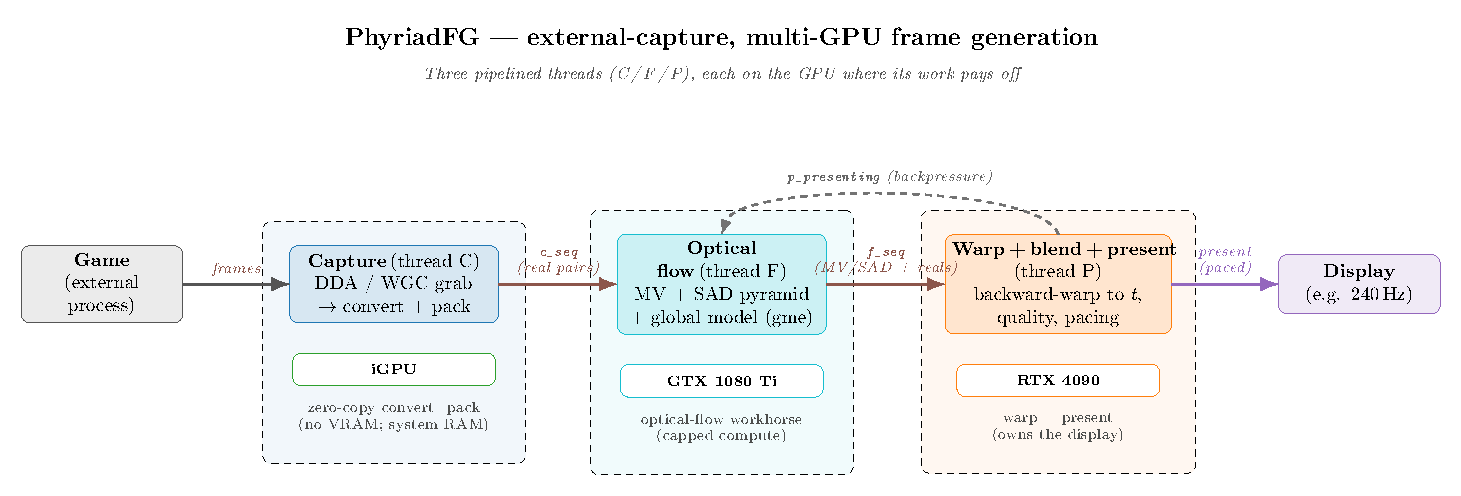
\includegraphics[width=\linewidth]{phyriadfg_multigpu.pdf}
\vfill
{\footnotesize Threads communicate through \texttt{FgContext} (SPSC rings + the sequence counters
\texttt{c\_seq} / \texttt{f\_seq} / \texttt{p\_presenting}); the present thread back-pressures the flow thread.}
\end{frame}

% ───────────────────────────────────────────────────────────────
\begin{frame}{How a frame is generated}
\centering
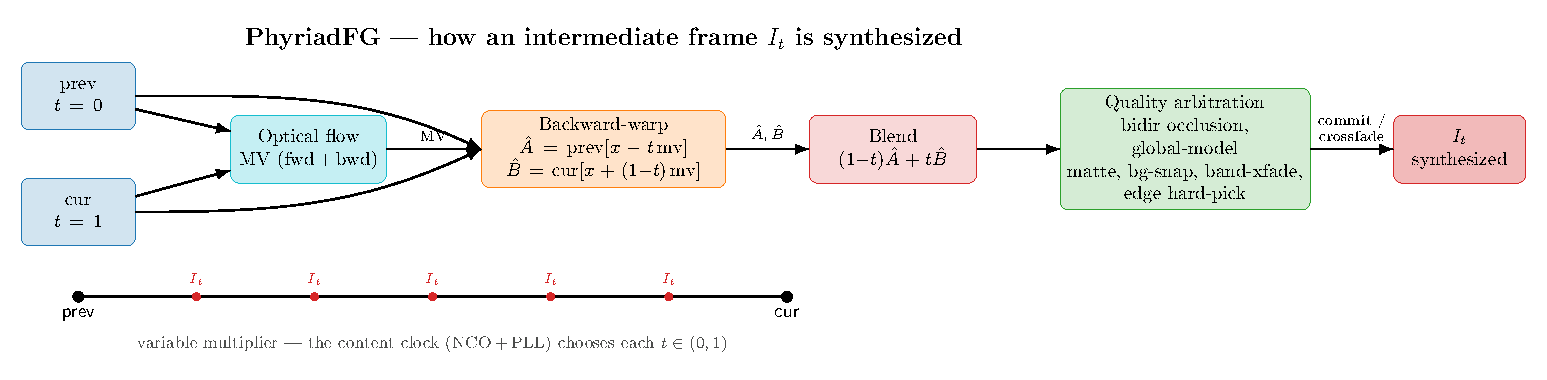
\includegraphics[width=0.96\linewidth]{phyriadfg_pipeline.pdf}
\vfill
{\footnotesize Backward-warp both reals to phase $t$, blend, then let the quality layers arbitrate the
hard cases (occlusion, disocclusion). The content clock chooses $t$ --- the multiplier is variable.}
\end{frame}

% ───────────────────────────────────────────────────────────────
\begin{frame}{Single source of truth --- the config resolver}
Flags parse into a \texttt{Config}; then \textbf{\texttt{resolve\_config()}} does, in \emph{one} place:
\begin{enumerate}
  \item \textbf{Dependency cascades} (order-independent): requires / disables / auto-enables.
  \item \textbf{Derived predicates} (\texttt{Config::Derived}): the single owner of cross-layer decisions ---
        e.g. \texttt{field\_to\_warp} = ``the iGPU contour field must reach the warp''. The create/import/upload
        sites read \emph{this}, instead of each re-deriving its own gate (which is how they drift).
  \item \textbf{A startup self-audit}: warns when a requested flag can have no effect (no silent no-ops).
\end{enumerate}
\vfill
{\footnotesize Idempotent + re-callable: a runtime degrade re-resolves in the same place. \textbf{To add a
capability that reads a shared resource, register it in the predicate --- the consumer sites never change.}}
\end{frame}

% ───────────────────────────────────────────────────────────────
\begin{frame}{Per-tick control --- the governor control word}
Under GPU saturation an optional governor graduates down non-essential work so the FG keeps generating.
The decision is \textbf{one control word, one owner}:
\begin{itemize}
  \item \texttt{governor\_floor\_for\_util()} --- the single decode of utilization $\to$ tier floor.
  \item \texttt{g\_gov\_floor} (atomic) --- \textbf{computed and published by the present thread} (it owns the
        utilization reading + hysteresis), \textbf{read by the flow thread} as \texttt{max(cpu\_ladder, floor)}.
  \item One producer, one consumer, advisory + lock-free. Governor off or GPU cool $\Rightarrow$ floor $0$ $\Rightarrow$ no-op.
\end{itemize}
\vfill
{\footnotesize One decode site, never two threads interpreting utilization independently.}
\end{frame}

% ───────────────────────────────────────────────────────────────
\begin{frame}{Quality layers (opt-in, composable)}
On top of the warp+blend core, each addressing a specific failure mode of external-capture interpolation:
\begin{columns}[T]
\column{0.5\textwidth}
\begin{itemize}\setlength\itemsep{2pt}
  \item bidirectional occlusion classification
  \item global affine motion model (gme) + matte
  \item background snap (kills disocclusion ``gravity'')
  \item band crossfade
\end{itemize}
\column{0.5\textwidth}
\begin{itemize}\setlength\itemsep{2pt}
  \item edge-gated hard-pick
  \item sub-pixel \& candidate-selected motion vectors
  \item object / scene holons (motion-inheritance repair)
  \item content-clock pacing, ASW extrapolation
\end{itemize}
\end{columns}
\vfill
{\footnotesize Each is a flag with a documented default; off paths are byte-identical. Composition is
resolved centrally (previous slide).}
\end{frame}

% ───────────────────────────────────────────────────────────────
\begin{frame}[fragile]{Build \& repository layout}
\begin{semiverbatim}\scriptsize
build.bat -> build\\phyriad_fg.exe        (MSVC + Vulkan SDK + Ninja, LTO)

src/core/      orchestrator: main, fg_context, globals, device, vk_util
src/cli/       Config + parsing + resolve_config (the resolver)
src/capture/   run_capture  [thread C]  DDA / WGC, convert/pack
src/flow/      run_flow     [thread F]  optical flow, gme, holons
src/warp_blend the warp-at-presenter + field/fill
src/present/   run_present  [thread P]  warp, quality, pacing, present
framework/     pillars: render/present, render/vulkan, hal, topology, schema
shaders/       the .comp shaders        ui/  Tauri launcher
\end{semiverbatim}
\end{frame}

% ───────────────────────────────────────────────────────────────
\begin{frame}{Honest scope}
\begin{itemize}
  \item \textbf{Is}: an external capture + interpolation + present pipeline, multi-GPU, with a quality stack
        for the hard cases and a launcher UI.
  \item \textbf{Is not}: an in-engine FG (no motion vectors / depth); it does not beat the display refresh
        without injection or a driver; it shares the GPU(s) with the game.
  \item \texttt{0.1.0-experimental}. Student-built, LLM-assisted. Numbers are stated only where measured.
\end{itemize}
\end{frame}

\end{document}
